\subsection*{V2. Weiss Molecular Field Theory|Exchange Field Theory|Curie Weiss Law}
\addcontentsline{toc}{subsection}{2. Weiss Molecular Field Theory|Exchange Field Theory|Curie Weiss Law}

This video is more about the introduction to Weiss Molecular Field Theory.
\begin{enumerate}
    \item In 1907, in order to explain spontaneous magnetization Weiss assumed that there exists an exchange field acting on a dipole which is given by:\\
    \begin{equation}
    \begin{split}
    H_{\mathrm{ex}} &= H_a + H_w \\
    H_{\mathrm{ex}} &= H + \lambda M
    \end{split}
    \end{equation}
    where $\mathrm{H_a}$ is the applied field, and $\mathrm{H_w}$ is the weiss field, and $\lambda$ is the Weiss constant.
    \item The Weiss field is proportional to its magnetization.
    \item Weiss constant determines the strength of the interaction of between the magnetic dipole moment in a material.
    \item In ferromagnetism, Curie law holds for exchange field as well.
\begin{figure}[htbp]
\centering
\begin{minipage}{0.55\textwidth}
\begin{equation}
\begin{split}
\chi &= \frac{C}{T} \\
\frac{M}{H_{\mathrm{ex}}} &= \frac{C}{T} \\
\frac{M}{H + \lambda M} &= \frac{C}{T} \\
M(T - \lambda C) &= C H \\
M &= \frac{C H}{T - C\lambda} \\
\chi &= \frac{C}{T - C\lambda}
\end{split}
\end{equation}

\vspace{0.5em}

\begin{equation}
\boxed{
\chi = \frac{C}{T - T_c}
}
\end{equation}
\end{minipage}
\hfill
\begin{minipage}{0.4\textwidth}
\centering
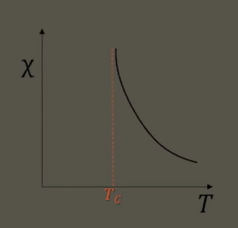
\includegraphics[width=\linewidth]{Images/Curie-weiss law.png}
\caption{Schematic graph of the Curie--Weiss law.}
\label{fig:curie-weiss-law}
\end{minipage}
\end{figure}
    \item This condition is only applicable above the transition temperature and this law is called as \hl{Curie-Weiss Law}.
    \item \textbf{Cases}:
    \begin{itemize}
        \item As $T\to T_c$, $\chi\to \infty$
        \item For $T<T_c$, Spontaneous magnetization exists, which means below the $T_c$ the material is acting as the ferromagnetic materials.
    \end{itemize}
    \item Temperature Dependence of Spontaneous Magnetization:
    \begin{itemize}
        \item Consider a spin system below $T_c$
        \item When $H=0$, \begin{equation}
            H_{ex}=\lambda M
        \end{equation}
        where $M=N\bar{\mu}$
    \end{itemize}
    \item According to quantum theory of paramagnetism, magnetization for spin half is;
\begin{figure}[htbp]
% \centering
\begin{minipage}{0.35\textwidth}
\begin{equation}
\begin{split}
M &= Ng\mu_B \tanh(x) \\
\mathrm{where}, g=1+\frac{J(J+1)+S(S+1)-L(L+1)}{2J(J+1)} \\
\mathrm{x}&= \frac{\mu_BgB}{\mathrm{k}T} \\
\end{split}
\end{equation}

\vspace{0pt}
\end{minipage}
\hfill
\begin{minipage}{0.3\textwidth}
\centering
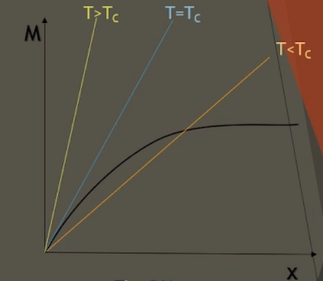
\includegraphics[width=\linewidth]{Images/temp_dependence.png}
\caption{Schematic graph of the temperature dependence of Curie-Weiss law.}
\label{fig:temperature dependence}
\end{minipage}
\end{figure}
\item In the case of ferromagnets we will have the nature of the plot as the $y=mx$ type plot. Only the different temperature will have different straight lines. $M=\left(\frac{kT}{\mu_0\mu_Bg\lambda}\right)x$. This is the final equation in the case of ferromagnets. 
\item As $T\uparrow,$ slope of straight line $\uparrow$.
\item For $T<T_c,$ two curves intersect which gives spontaneous magnetization. [\textcolor{red}{Q.When is the spontaneous magnetization is going to be maximum?}]
\item Maximum spontaneous magnetization occurs at $T=0$ K.
\item At $T=T_c,$ straight line is tangential to hyperbolic curve at origin.
\item For $T>T_c,$ spontaneous magnetization remains zero.
\item For normalized magnetization, the thermomagnetic equation of the state for ferromagnetic phase, is given by;
\begin{equation}
 \begin{split}
   \frac{Ms(T)}{M_s(0)}=\frac{Ng\mu_B \tanh{(T/T_c)}}{Ng\mu_b}\\
   \frac{Ms(T)}{M_s(0)}=\tanh{(T/T_c)}
 \end{split}    
\end{equation}
\end{enumerate}